\documentclass[mathserif, aspectratio=169]{beamer}
\usetheme{odenpecos}
\setbeamertemplate{itemize/enumerate body begin}{\fontsize{8.8}{9}\selectfont}
\setbeamertemplate{itemize/enumerate subbody begin}{\fontsize{7.5}{8}\selectfont}
\setbeamertemplate{itemize/enumerate subsubbody begin}{\fontsize{7.5}{8}\selectfont}

% default search path for figures
\graphicspath{{../fig/}}

\newcommand{\zapspace}{\topsep=0pt\partopsep=0pt\itemsep=0pt\parskip=0pt}

\usepackage{multicol}
\usepackage{pict2e}
%\usepackage{esdiff}
\usepackage{multimedia}
\usepackage{verbatim}
\usepackage{mhchem}
\usepackage{tikz}
\usetikzlibrary{arrows}
\usepackage[percent]{overpic}
\usepackage[absolute,overlay]{textpos}
\usepackage{tikz} % Required for flow chart
\usepackage[caption=false]{subfig}

\newcommand{\overbar}[1]{\mkern 1.5mu\overline{\mkern-1.5mu#1\mkern-1.5mu}\mkern 1.5mu}
\newcommand{\pp}[2]{\frac{\partial #1}{\partial #2}}
\newcommand{\dd}[2]{\frac{d #1}{d #2}}
\newcommand{\DD}[2]{\frac{D #1}{D #2}}
\newcommand{\mm}{\mathbf{minmod}}
\def\etal{{\it et al~}}
\newcommand{\be}{\begin{eqnarray}}
	\newcommand{\ee}{\end{eqnarray}}
\newcommand{\mbb}[1]{\mathbb{#1}} % math blackboard bold
\newcommand{\mcal}[1]{\mathcal{#1}} % math blackboard bold
\newcommand{\mbf}[1]{\mathbf{#1}} % math bold face (for vectors)
\newcommand{\sbf}[1]{\boldsymbol{#1}} % bold face for symbols
\newcommand{\jump}[1]{\llbracket #1 \rrbracket} % jump operator
\newcommand{\avg}[1]{\langle #1 \rangle} % average operator
\newcommand{\rarrow}{\rightarrow}
\newcommand{\Rarrow}{\Rightarrow}
\newcommand{\LRarrow}{\Leftrightarrow}
\newcommand{\vvvert}{|\kern-1pt|\kern-1pt|}
\newcommand{\enorm}[1]{\vvvert #1 \vvvert}
\newcommand{\nutil}{\tilde{\nu}}
\newcommand{\Var}{\mathrm{Var}}
\newcommand{\Cov}{\mathrm{Cov}}


\definecolor{MyDarkGreen}{rgb}{0,0.45,0.08}
\newcommand{\myred}[1]{{\color{red} #1}}
\newcommand{\myblue}[1]{{\color{blue} #1}}
\newcommand{\mygreen}[1]{{\color{MyDarkGreen} #1}}

\newcommand{\sa}{\nu_{\mathrm{sa}}}
\newcommand{\tep}{\tilde{\epsilon}}
\newcommand{\Ssd}{\mathcal{S}} % source term due to slow derivative
\newcommand{\ud}{\,\mathrm{d}}

\newcommand{\Mach}[1]{\ensuremath{\mbox{Ma}_{#1}}}
\newcommand{\Reynolds}{\ensuremath{\mathit{Re}}}
\newcommand{\DensityRat}{\ensuremath{\mathit{DR}}}
\newcommand{\BlowRat}{\ensuremath{\mbox{BR}}}
\newcommand{\VelRat}{\ensuremath{\mathit{VR}}}
\newcommand{\Tau}{\ensuremath{\mathrm{T}}}

\newcommand{\wall}     {\ensuremath{\mathrm{w}}}   % wall subindex
\newcommand{\awall}    {\ensuremath{\mathrm{aw}}}  % adiabatic wall subindex

\newcommand{\commentout}[1]{}

\newcommand{\vect}[1]{\boldsymbol{#1}}
\usepackage{mleftright}
\newcommand{\of}[1]{\mleft( #1 \mright)}
\newcommand{\vth}{v_{\textrm{th}}}
\newcommand{\reals}{\mathbb{R}}
\newcommand{\myint}{\int\limits}
\newcommand{\ddt}[1]{\partial_t #1}
\newcommand{\RR}{\mathbb{R}}
\newcommand{\vr}{v}
\newcommand{\diff}[1]{\, d#1}
\newcommand{\norm}[1]{\left\lVert#1\right\rVert}
%\newcommand{\vtheta}{\theta_{\vect{v}}}
%\newcommand{\vphi}{\varphi_{\vect{v}}}
%\newcommand{\vr}{v_{r}}
\newcommand{\vtheta}{{v_{\theta}}}
\newcommand{\vphi}{v_{\varphi}}
\newcommand{\vomega}{v_{\omega}}
\newcommand{\vrunit}{\hat{\vect{v}}_{r}}
\newcommand{\vthetaunit}{\hat{\vect{v}}_{\theta}}
\newcommand{\vphiunit}{\hat{\vect{v}}_{\varphi}}
\DeclareMathOperator{\variance}{Var}

\begin{document}
% disable nav
\setbeamertemplate{navigation symbols}{}

% ---------------------------------------------------------------
% Oden/Pecos title page

\hoffset=.16in

\begin{frame}[plain,t]{}
\makeatletter
%\vspace*{0.85cm}
%\vspace*{0.65cm}
\includegraphics[height=0.9in,trim=50 40 40 0, clip]{PMSc_159_university_formal_horizontal.pdf} \newline
%\vspace*{0.3cm}
\begin{columns}[T,onlytextwidth]
\column{.8\textwidth}
{\bf \color{burntorange} \fontfamily{bch}\selectfont 
% -- Set talk title here
Solving the Boltzmann equation for electron kinetics using Galerkin approach
% --
}
\end{columns}
\vspace*{.15cm}
\rule{.8\textwidth}{0.6pt} \newline

\vspace*{0.05cm}
\setstretch{0.65}
{\fontfamily{phv}\selectfont
  { \scriptsize
    % -- define presenter, authors here
    Milinda Fernando, Daniil Bochkov, Todd Oliver, Laxminarayan Raja, Philip Varghese, Robert Moser, George Biros  \\
    % --
  }
  {\color{burntorange} \tiny
    % -- define role, meeting event, location, etc
    PSAAP III Annual Review $\cdot$ November 03-04, 2022
    % --
  }
}

\vspace*{1cm}
%\includegraphics[height=0.3in]{figures/pecos_orange1.png}
\begin{columns}
\begin{column}{0.8\linewidth}
\includegraphics[height=0.5in]{oden_pecos_2020_wordmark.png}\\
{\scriptsize \url{https://pecos.oden.utexas.edu}}
\end{column}

\begin{column}{0.2\linewidth}
\includegraphics[height=0.6in]{psaap3-logo.png}
\end{column}
\end{columns}

\end{frame}
\hoffset=0in
% -- end title slide ---------------------------------------------

%\begin{frame}
%	\frametitle{Outline}
%	\begin{itemize}
%		\item Spatially homogeneous Boltzmann equation, $\partial_t f - \frac{\vect{E} q}{m} \cdot \nabla_{\vect{v }}f = C(f)$
%		\item Representation of $f$ (i.e., isotropic + anisotropic correction terms), use spherical harmonics for angular directions + experimentation of basis functions in radial direction. 
%		\begin{itemize}
%			\item Global approximations with Maxwell and Laguerre polynomials.
%			\item Local approximations with linear and higher order B-splines
%		\end{itemize}
%		\item Collision operator (5d integral form)
%		\item Simplifications for the collision operator with analytical integration of angular directions (1d integral form). 
%		\item Equations for the steady-state solution (spatially homogeneous case) 
%		\item Two-term formulation vs. EEDF formulation with diffusion term. 
%		\item Verification with Bolsig+ code.  (Both approaches, importance of the diffusion term), PS 2.4
%		\item Formulation for 1D-space+3D-velocity space Boltzmann equations with some preliminary results for 1d glow discharge problem. 
%		\item Discuss on single GPU implementation with CuPy, Challenges in 1D+3V formulation (i.e., boundary conditions) and Future work, ES 2.6
%	\end{itemize}
%\end{frame}

\begin{frame}[fragile]
	\frametitle{Where do we fit ? }
	% \begin{tikzpicture}
	% 	\node[anchor=south west,inner sep=0] at (0,0) {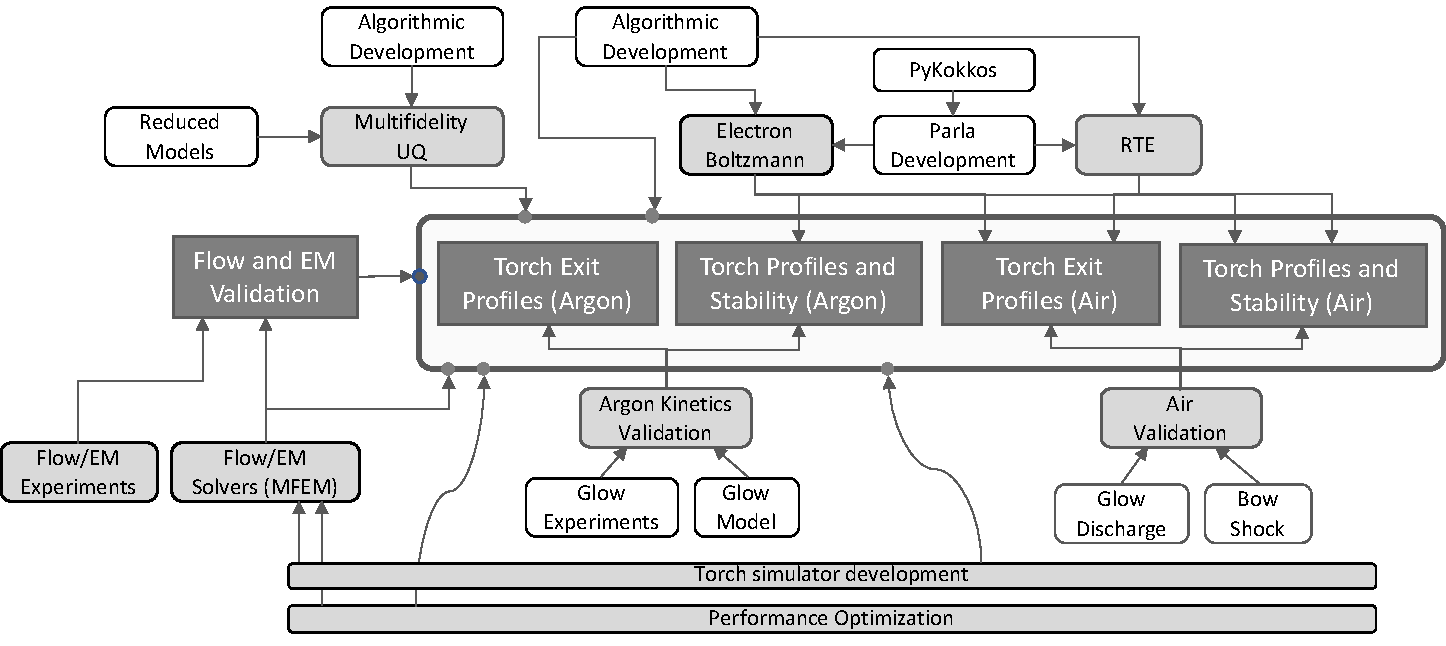
\includegraphics[width=0.8\textwidth]{pecos_roadmap_tst_1.5.pdf}};
	% 	\draw[orange, fill = yellow!30, fill opacity = 0.4 ,ultra thick,rounded corners] (4.15,3.6) rectangle +(4.2,1.6);
	% \end{tikzpicture}
	\begin{center}
		\includegraphics[width=0.8\textwidth]{road_map.png}
	\end{center}
\end{frame}

\begin{frame}
	\frametitle{Outline}
	\begin{itemize}
		\item 0D3V - Homogeneous in space
		\begin{itemize}
			\item Formulation
			\item Discretization
			\item Results
			\item Verification with Bolsig+
		\end{itemize}
		\item 1D3V - Glow discharge problem
		\begin{itemize}
			\item Formulation
			\item Discretization
			\item Boundary conditions
		\end{itemize}
		\item Future work
	\end{itemize}
	% \begin{itemize}
	% 	\item Current work on deterministic Boltzmann solver for 0D3V and 1D3V
	% 	\begin{itemize}
	% 		\item 0D3V solver
	% 		\begin{itemize}
	% 			\item Studied efficient discretization in speed
	% 			\item Verified 0D3V code with Bolsig+ in different parameter regimes
	% 		\end{itemize}
	% 		\item 1D3V solver
	% 		\begin{itemize}
	% 			\item Implemented CPU/GPU Python implementation
	% 			\item Currently, resolving issues with boundary conditions
	% 		\end{itemize}
	% 	\end{itemize}
	% 	\item 0D3V formulation and results
	% 	\item 1D3V formulation and preliminary results
	% \end{itemize}
\end{frame}

\begin{frame}
	\frametitle{0D3V - Boltzmann equation}
	\begin{itemize}
		\item For a given electric field $\vect{E}$
		\begin{align}
			\partial_t f -\frac{\vect{E} q}{m} \cdot \nabla_{\vect{v }}f = C(f)
		\end{align} 
		\item Derived the steady state equation
		\begin{align}
			\textcolor{black!70}{\partial_t \hat{f} = -(u^T C \hat{f}) \hat{f} + (C+E)\hat{f} \text{ where } \hat{f}(\vect{v},t) = \frac{f(v,t)}{\myint_{R^3} f(\vect{v},t) \diff{\vect{v}}}}\\
			\textcolor{black!70}{\partial_t (\hat{f}) = 0 \ \ \  \Rightarrow} \ \ \  -(u^T C \hat{f}) \hat{f} + (C+E)\hat{f} =0  \text{ with } u^T \hat{f}-1=0
		\end{align}
	\end{itemize}
\end{frame}

\begin{frame}
	\frametitle{0D3V - Challenges}
	\begin{columns}
		\begin{column}{0.45\textwidth}
			\begin{itemize}
				\item Non-smooth cross sections $\Rightarrow$ non-smooth solutions
				\item Strong advection causes stabilization issues
				\item To capture reaction rates needs accurate tail representations of $f$
				\item Need compact representation of $f$ (for 3D3V case)
			\end{itemize}
		\end{column}
		\begin{column}{0.45\textwidth}
			\begin{center}
				\includegraphics[width=1.2\columnwidth]{g0_g2_cs.png}
			\end{center}
		\end{column}
	\end{columns}
\end{frame}

\begin{frame}
	\frametitle{0D3V - Discretization}
	\small
	\begin{itemize}
		\item Representation of $f$
		\begin{itemize}
			\item $\Phi_k\of{v}$ : Global polynomials
			\item $\Phi_k\of{v}$ : Local B-splines
			$
			\displaystyle
			\quad 
			f(\vect{v},t) = \sum_{klm} f_{klm} \underbrace{\Phi_k\of{v}}_{\text{radial basis}} \underbrace{Y_{lm}\of{v_\theta, v_\phi}}_{\tiny\text{sph. harm.}}$ 
			%with $
			% \displaystyle
			% \quad 
			% \phi_{pqs}\of{\vect{v}} = \underbrace{\Phi_p\of{v}}_{\text{radial basis}} \underbrace{Y_{qs}\of{v_\theta, v_\phi}}_{\tiny\text{sph. harm.}}$
		\end{itemize}
		\item Weak formulation
			$
			\displaystyle
			\quad
			\partial_t f - \frac{\vect{E} q}{m} \cdot \nabla_{\vect{v}}f = C(f)
			\quad $ \\
			$
			\displaystyle
			\quad
			\Rightarrow \quad
			\partial_t \myint_{R^3} f \phi\of{\vect{v}} \ud \vect{v} = 
			\myint_{R^3} C(f) \phi\of{\vect{v}} \ud \vect{v} + \myint_{R^3} \of{\frac{\vect{E} q}{m} \cdot \nabla_{\vect{v}} f} \phi(\vect{v}) \ud \vect{v}\text{ , } 
			\forall \phi(\vect{v})$
		\item Weak form of the collision operator \\
			$
			\displaystyle
			\quad 
			\myint_{R^3} C \phi\of{\vect{v}_e} \diff{\vect{v}_e} 
			=
			N \myint_{R^3} \myint_{S^2} 
			v\sigma(v,\vect{\omega})
			f_e\of{\vect{v}_e}
			\left(
			\phi\of{\vect{v}_e^\text{post}\of{\vect{v}_e, \vect{\omega}}} 
			- \phi\of{\vect{v}_e} 
			\right)
			\diff{\vect{v}_e} \diff{\vect{\omega}}
			$
	\end{itemize}
\end{frame}

\begin{frame}
	\frametitle{0D3V - R\&D activities}
	% \begin{tabular}{l|c|c|l}
	% 	\hline \\
	% 	Activity & Conclusion \\
	% 	\hline
	% 	Local and global basis representations & Local representation perform better capturing non-smooth $f$ and discontinuous cross sections \\
	% 	Non-uniform grids in radial direction  & Did not make much difference in the DOFs used. \\
	% 	Discontinuous and continuous Galerkin approaches & Deriving the coupling terms for the collision operator is bit trickly for the DG formulation. \\
	% 	Lagrange and Eulerian approaches for advection & Eulerian approach seems to work fine, we can capture $f$ with few $l$ (polar) modes. \\
	% 	Simplifying collision operator  & Simplifications with EEDF formulations gave use better tail representations.	\\
	% 	Validation with state-of-the-art Bolsig+ code	& We show good agreement with steady-state solutions computed with Bolsig+ code. \\
	% 	\hline
	% \end{tabular} 
	\begin{itemize}
		\item Local and global basis representations for $\Phi_k\of{v}$
		% \begin{itemize}
		% 	\item Local representation perform better capturing non-smooth $f$ and discontinuous cross sections
		% \end{itemize}
		
		\item Radially non-uniform discretization
		% \begin{itemize}
		% 	\item Not a significant difference in the DOFs required
		% \end{itemize}

		% \item Discontinuous and continuous Galerkin approaches
		% \begin{itemize}
		% 	\item Deriving the coupling terms for the collision operator is bit trickly for the DG formulation.
		% \end{itemize}

		\item Lagrange and Eulerian approaches for advection
		% \begin{itemize}
		% 	\item Eulerian approach seems to work fine, we can capture $f$ with few $l$ (polar) modes. The advection operator will trigger spherical asymmetry, while the collision operator kills it
		% \end{itemize}

		\item Verification with Bolsig+\footnote[frame]{Hagelaar, G.J.M. and Pitchford, L.C., 2005. Solving the Boltzmann equation to obtain electron transport coefficients and rate coefficients for fluid models. Plasma sources science and technology, 14(4), p.722.}, fixed two term approximation $f(\vect{v},t) = f_0(v, t) + f_1(v,t)\cos v_\theta$
		% \begin{itemize}
		% 	\item We show good agreement with steady-state solutions computed with Bolsig+ code.
		% \end{itemize}

		\item Implemented Bolsig code two term approximation, with simplified collision operator
		% \begin{itemize}
		% 	\item Simplifications with EEDF formulations gave use better tail representations.
		% \end{itemize}
	\end{itemize}
\end{frame}

\begin{frame}[fragile]
	\frametitle{Global vs. Local Galerkin approximations}\
	\vspace{-0.5in}
	\begin{figure}
		\subfloat[\tiny{Maxwell polynomials, E=200 V/m, with elastic + ionization }]{%
			\includegraphics[width=0.8\textwidth]{maxwell_E200_g0g2.png}
		}\\
		\subfloat[\tiny{B-Splines, E=200 V/m, with elastic + ionization }]{%
			\includegraphics[width=0.8\textwidth]{bspline_sp2_E200_g0g2.png}
		}
	\end{figure}
\end{frame}

\begin{frame}
	\frametitle{Bolsig+ collision operator}
	\begin{columns}
		\begin{column}{\textwidth}
			\begin{itemize}
				\item Bolsig only use 2 $\vtheta$ terms: $1, \cos\vtheta$ and constant in $\vphi$ direction. 
				%We assume azimuthal symmetry for the time-being, $lm=\{(0,0), (1,0), (2,0), ...\}$
				% \item $\vect{v}^{\prime} = (v_r^\prime, v_\theta^\prime, v_\phi^\prime) =\vect{v}^{post}\of{\vect{v},\vect{0},\vect{\omega}}$
				% \begin{align*}
				% 	\cos v_\theta^\prime = \cos v_\theta \cos\chi + \sin v_\theta \sin \chi \cos\of{v_\phi-\phi}
				% \end{align*}
				\item Simplified collision operator, $f(v,\vtheta,\vphi) = f_0(v) + f_1(v) \cos\vtheta$ with $\hat{f}_{0,1} = \cfrac{f_{0,1}}{n_e}$
				%Using the spherical harmonics addition theorem and integrating out the angles analytically, 
				% \begin{align*}
				% 	P_l^{0} = P_l\of{\cos v_\theta^\prime} =  P_l\of{\cos v_\theta} P_l\of{\cos v_\phi} + 2\sum_{m=1}^{l} P_l^{m}\of{\cos v_\theta} P_l^{m}\of{\cos v_\phi} \cos \of{ m (v_\phi-\phi)}
				% \end{align*}
				% \item Analytically integrating out the angles, we can write,
				\begin{align}
					\myint_{v} C \psi\of{v} \diff{v}  = N \myint_{v} v^3 \sigma\of{v} f_l\of{v} \delta_{ql} \of{\psi\of{v^{post}}\delta_{q0} - \psi\of{v}} \diff{v}  
				\end{align}
				\item Steady state equations becomes (assuming $l=0,1$ and $m=0$ modes), 
				\begin{align}
					&\frac{E^2}{3} \partial_{v} \of{\frac{\partial_v \hat f_0}{(N \varepsilon^{1/2}\gamma \sigma\of{\varepsilon} + \mu)}} + \frac{2E^2}{3v} \frac{\partial_v \hat{f_0}}{(N \varepsilon^{1/2}\gamma \sigma\of{\varepsilon} + \mu)} + \tilde C_0 \hat{f_0} = \mu \hat{f_0} \\
					&\hat{f_1} = \frac{E}{\sqrt{3}} \frac{\partial_{v}\hat{f_0}}{(N \varepsilon^{1/2}\gamma \sigma\of{\varepsilon} + \mu)}
				\end{align}
				\item Only solve for $\hat{f}_0$ and $\hat{f}_1$ is derived from $\hat{f}_0$ as above
			\end{itemize}
		\end{column}
		% \begin{column}{0.48\textwidth}
			
		% \end{column}
	\end{columns}
\end{frame}

\begin{frame}
	\frametitle{B-Splines + EEDF formulation + simplified collision op + Galerkin approximation}
	\begin{figure}
		\subfloat[\tiny{B-Splines, E=200 V/m, with elastic + ionization with EEDF formulation}]{%
			\includegraphics[width=0.99\textwidth]{bspline_sp2_E200_g0g2_eedf.png}
		}
	\end{figure}
\end{frame}

\begin{frame}
	\frametitle{Global vs. Local basis approximations}
	\begin{itemize}
		\item Global polynomials (Maxwell, Laguerre, Chebyshev)
		\begin{itemize}
			\item Pros
			\begin{itemize}
				\item Spectral convergence
				\item Work well with highly smoothed cross-sections
			\end{itemize}
			\item Cons
			\begin{itemize}
				\item \textcolor{orange}{Computed operators are sensitive to chosen thermal velocity}
				\item With LXCAT data tails are not well resolved 
				\item Ionization and excitations cross sections are non-smooth%Struggle to capture sharp variations in $f$
			\end{itemize}
		\end{itemize}
		\item Local approximations with B-Splines
		\begin{itemize}
			\item Pros
			\begin{itemize}
				\item Flexibility in quadrature, and knot placement
				\item Tails are better resolved compared to the global approximations
			\end{itemize}
			\item Cons
			\begin{itemize}
				\item Lower-order convergence
			\end{itemize}
		\end{itemize}
	\end{itemize}
	\begin{itemize}
		%\item Lower order splines, simplified collision operator with EEDF formulation seems to capture tails better compared to previous cases
		\item Lower order splines seems to capture tails better 
		\item For time-being we are planning to move forward with low-order B-Spline approximations 
	\end{itemize}
\end{frame}

\begin{frame}
	\frametitle{Comparison with Bolsig+ Nr=128}
	\begin{center}
		\only<+>{
			\begin{itemize}
				\item Elastic reaction rates
			\end{itemize}
			\includegraphics[width=0.48\textwidth]{pde_vs_bolsig_collop_approx_eedf_g0.png}
			\includegraphics[width=0.48\textwidth]{pde_vs_bolsig_collop_approx_eedf_g0_rerror.png}
			}
		\only<+>{
			\begin{itemize}
				\item Ionization reaction rates
			\end{itemize}
			\includegraphics[width=0.48\textwidth]{pde_vs_bolsig_collop_approx_eedf_g2.png}
			\includegraphics[width=0.48\textwidth]{pde_vs_bolsig_collop_approx_eedf_g2_error.png}
			}
		\only<+>{
			\begin{itemize}
				\item Steady-state energy
			\end{itemize}
			\includegraphics[width=0.48\textwidth]{pde_vs_bolsig_collop_approx_eedf_energy.png}
			\includegraphics[width=0.48\textwidth]{pde_vs_bolsig_collop_approx_eedf_energy_rerror.png}
			}
	\end{center}
\end{frame}

\begin{frame}
	\frametitle{Glow Discharge with 1D3V Boltzmann}
	\begin{align}
		&\partial_t f + v\cos\of{\vtheta} \partial_z f -\vect{E}\cdot\nabla_v f = C[f] \text{ for } (z,\vect{v}) \in (0,L) \times R^3 \\
		&\textcolor{red!80}{f(\vect{v}, 0, t, \vtheta \leq \frac{\pi}{2})	= 0 \text{ and } f(\vect{v}, L, t, \vtheta > \frac{\pi}{2})	= 0}\\
		&\partial_t n_i + \partial_z \of{\mu_i n_i E\of{z,t} -D_i \partial_z n_i} = N \gamma \myint_{\varepsilon}\myint_{\vect{\omega}} \varepsilon^{1/2} \sigma_i f d\vect{\omega} d\varepsilon \\
		& \vect{E} = \nabla \of{\Delta^{-1}\frac{e}{\epsilon_0} \of{n_i- n_e}} \text{ , } n_e = \myint_{\vect{v}} f\of{\vect{v}, z, t} \diff{\vect{v}}
	\end{align}
	
	\begin{itemize}
		\item 1D3V - Challenges
		\begin{itemize}
			\item The spatial boundary conditions are discontinuous in $\vtheta$ $\Rightarrow$ will increase the number of $l$ modes required
			\item Periodic solution in time $\Rightarrow$ requires timestepping, no direct steady state solutions
		\end{itemize}
	\end{itemize}
\end{frame}

\begin{frame}
	\frametitle{1D3V - Discretization}
	\begin{itemize}
		\item Use method of discrete ordinates in $\vtheta$, $f_{\vtheta_j} = f(v, \vtheta_j, z, t)$
		\begin{align}
			\partial_t f_{\vtheta_j} + v\cos\of{\vtheta_j} \partial_z f_{\vtheta_j} = P_{\vtheta_j} (C + E) \begin{bmatrix}
				f_{\vtheta_0}\\
				\vdots\\
				f_{\vtheta_{N_\vtheta}}\\
			\end{bmatrix} ; j=1,..., N_{\vtheta}
		\end{align}
		\item Use B-splines + spherical basis representation of $f$ in the velocity-space for collision and v-space advection
		\item Use finite difference method in $z$ direction
		\item Use method of lines + with explicit time integrator in time
		\item First order explicit operator splitting for evolving $n_i$ and $\vect{E}$ field equations
	\end{itemize}
\end{frame}

\begin{frame}
	\frametitle{1D3V - Results}
	\begin{center}
		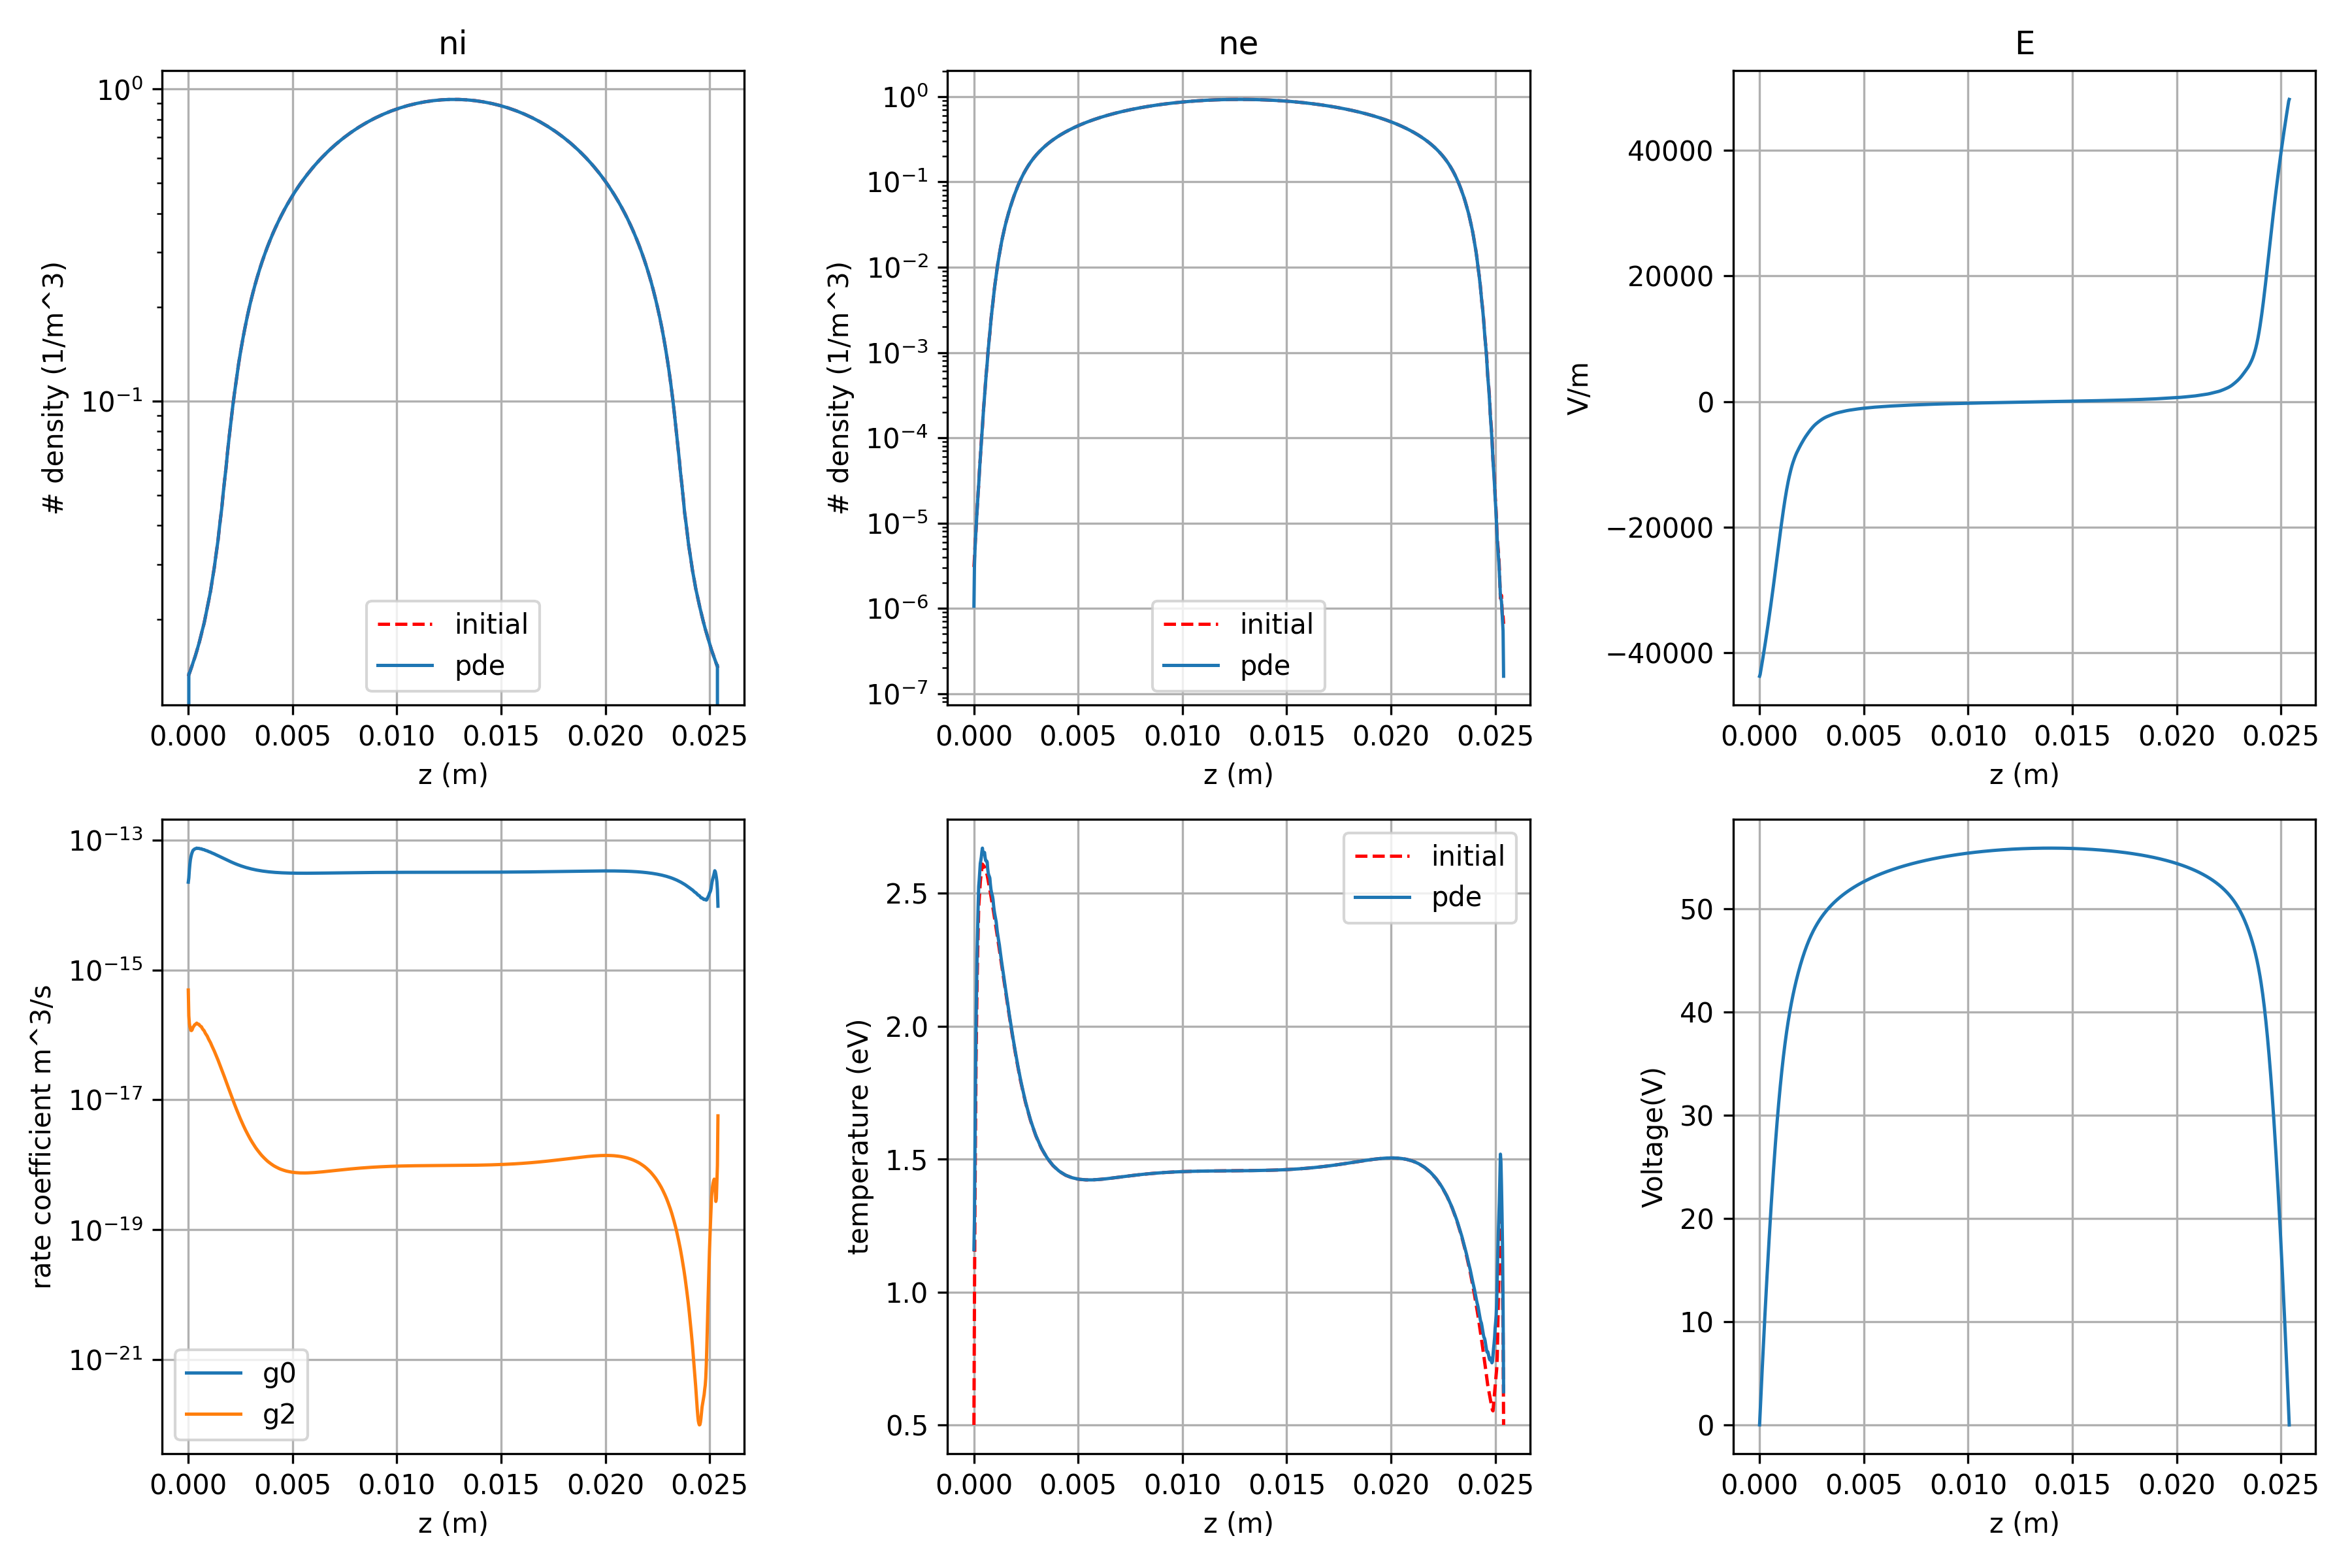
\includegraphics[width=0.6\textwidth]{glow_discharge_1d3v_g0_g2_v0_z01.0_E0.0_poly_bspline_sp_2_nr128_lmax3_qpn4_ev2.000000E+00_bscale1.0_dt1.0000E-13_T1.00E-10_qoi.png}
	\end{center}
	\begin{itemize}
		\item Currently, instabilities on the boundary propagate inwards.
	\end{itemize}
\end{frame}

\begin{frame}
	\frametitle{Future work}
	\begin{itemize}
		\item Add filtering in $\vtheta$ direction
		\item Supports adaptive discrete ordinates in space
		\item Integration with PyKokos and Parla
		\item Revisit radial discretization
		\begin{itemize}
			\item DG or finite volume discretization
		\end{itemize}
		\item Artificial diffusion in speed, for stabilization ?
	\end{itemize}
\end{frame}

\begin{frame}
	\centering
	\Huge Questions ? \\
	\centering
	\Huge Thank You. 
\end{frame}


\end{document}
